\documentclass{article}

\usepackage[paper=letterpaper,margin=2.5cm]{geometry} % Set Margins

%% Math and math fonts
\usepackage{amsmath, amsthm, amssymb, amsfonts}
\usepackage{bbm} % for \mathbbm{1}

% date
\usepackage[nodayofweek]{datetime}

% Color
\usepackage{color, xcolor}

% Misc
\usepackage{environ}  % \collect@body in asmmath
\usepackage{graphicx} % \includegraphics options
\usepackage{mdframed} % text boxes
\usepackage{indentfirst} % Indent first paragraph after section header
\usepackage[shortlabels]{enumitem} % Control enumerate items with [(a)]
\usepackage{comment} % Comments
\usepackage{fancyhdr} % Headers and footers

% Tables
\usepackage{array}

% Sub-figures and figure placement
\usepackage{caption}
\usepackage{subcaption}
\usepackage{float} 

% Graphing
\usepackage{pgfplots}
\pgfplotsset{compat=1.17}
\usepackage{tikz}

% Title Placement
\usepackage{titling}
\setlength{\droptitle}{-6em}

%set indent to 
\setlength{\parindent}{0pt}

% Hyper refs
\usepackage{hyperref}
\hypersetup{
    colorlinks=true,
    linkcolor=blue,
    urlcolor  = blue,
    filecolor=magenta,      
    urlcolor=blue,
    citecolor = blue,
    anchorcolor = blue
}

% % Citation management
\usepackage{natbib}
\bibliographystyle{abbrvnat}
\setcitestyle{authordate,open={(},close={)}}

\pagestyle{fancy}

\usepackage[paper=letterpaper,margin=2.5cm]{geometry} % Set Margins

%% Math and math fonts
\usepackage{amsmath, amsthm, amssymb, amsfonts}
\usepackage{bbm} % for \mathbbm{1}

% date
\usepackage[nodayofweek]{datetime}

% Color
\usepackage{color, xcolor}

% Misc
\usepackage{environ}  % \collect@body in asmmath
\usepackage{graphicx} % \includegraphics options
\usepackage{mdframed} % text boxes
\usepackage{indentfirst} % Indent first paragraph after section header
\usepackage{comment} % Comments
\usepackage{fancyhdr} % Headers and footers

% Tables
\usepackage{array}

% Sub-figures and figure placement
\usepackage{caption}
% \usepackage{subcaption}
\usepackage{float} 

% Graphing
\usepackage{pgfplots}
\pgfplotsset{compat=1.17}
\usepackage{tikz}

% Title Placement
\usepackage{titling}
\setlength{\droptitle}{-6em}

%set indent to 
\setlength{\parindent}{0pt}

% Hyper refs
\usepackage{hyperref}
\hypersetup{
    colorlinks=true,
    linkcolor=blue,
    urlcolor  = blue,
    filecolor=magenta,      
    urlcolor=blue,
    citecolor = blue,
    anchorcolor = blue
}

% % Citation management
\usepackage{natbib}
\bibliographystyle{abbrvnat}
\setcitestyle{authordate,open={(},close={)}}

\newcolumntype{M}{>{$}c<{$}} % Define a new column type for math mode


% ----------------------------------------
% TITLE
% ----------------------------------------

\pagestyle{fancy}

\lhead{Creel}
\chead{Differential Equations}
\rhead{AMES}

\title{AMES Class Notes -- Week 11, Monday: Differential Equations}
\author{Andie Creel}

\begin{document}
\maketitle

\section{Introducing terms}
Think if you have rabbits and they are breading in different time periods 

\begin{center}
    \begin{tabular}{ c c c c}
     row & Time period (t) & number of rabbits (x) & number of rabbits written differently \\
     1 & 0 & 2 & $x_0$\\ 
     2 & 1 & 8*2 & $8* x_0$\\  
     3 & 2 & 8*8*2 & $8*x_1$  \\
     4 & 3 & 8*8*8*2 & $8* x_2$
    \end{tabular}
\end{center}

\textbf{Recursion equations }(the state today depends on the state before): 
\[x_{t+1} = x_t + f(x_t)\]

\textbf{Difference equation: }
\[\frac{\Delta x}{\Delta t} = x_{t+1} - x_t = f(x_t)\]

\textbf{Differential equation:} Notice that we currently have the difference equation written for discrete time. Let's take a limit the limit to get it to continuous time. This is what makes a \textit{difference} equation a \textit{differential equation}, where the state $x$ is a function of the time period $t$, $x(t)$ (\textbf{time non-autonomous}). 
\begin{align}
    \Delta t \rightarrow 0\\
    \dot x = \frac{\partial x(t)}{\partial t} = f(x(t)) = f(x, t). \label{nonauto}
\end{align}
In this case, the time period $t$ genuinely matters  For example, if you run a Christmas tree farm, the date may really matter. This is what it is why it's time \textit{non}-autonomous. \\


Alternatively, we can suppress the $t$ and instead just focus on the state of the world, regardless of the time period (\textbf{time autonomous})
\begin{align}
    \dot x = \frac{\partial x}{\partial t} = f(x) \label{auto}
\end{align}

Sometimes the system we're interested in will be \textit{time autonomous} meaning that the year or date doesn't really matter. It's just the state of the world that matters. \\

In conclusion, sometimes time may really matter, where the time period does affect the the state of the world directly (like in equation \ref{nonauto}). For instance, if we're interested in a seasonal patter, the time will matter. However, if we're just interested in what people do on warm days, it does \textit{not} matter if that warm day happens in the summer or if it's random very warm day in the fall (like in equation \ref{auto}). 

\section{Using differential equation to get x(T)}

Let's say we know how the stock $x_t$ changes through time, and we know the stock level in time period $0$, $x_0$. \textbf{We want to know the stock level in time period $T$, $x(T)$}

\begin{align*}
    \frac{\partial x(t)}{\partial t} = a + bx(t)
\end{align*}

If we want the level instead of the change we can integrate. Let's also get rid of the fractions. 

\begin{align*}
    \partial x(t) = (a + b x(t)) \partial t
\end{align*}

Let's rename $x(t) = z$ to get rid of the $t$. 

\begin{align}
    \partial z = (a + b z) \partial t
\end{align}

Let's get all the $z$ on the same time 
\begin{align*}
    \frac{\partial z}{a + b z} = \partial t
\end{align*}

\textbf{We've seperated variables}. Now let's integrate. 

\begin{align*}
    \int_{x(0)}^{x(T)} \frac{\partial z}{a + b z} &= \int_0^T \partial t\\
     \int_{x(0)}^{x(T)} \frac{\partial z}{a + b z} &= \int_0^T \partial t\\
     \int_{x(0)}^{x(T)} \frac{\partial z}{a + b z} &= t|_0^T \\
     \int_{x(0)}^{x(T)} \frac{\partial z}{a + b z} &= T \\
     \int_{x(0)}^{x(T)} \frac{1}{a + b z} \partial z &= T
\end{align*}

Now, we need to do a u-sub. 
\begin{align*}
    u &= a + bz\\
    \frac{\partial u}{\partial z} &= b \implies dz = du / b\\
    \int_{x(0)}^{x(T)} \frac{1}{u} \frac{du}{b} &= T \\
    \frac{1}{b }\int_{x(0)}^{x(T)} \frac{1}{u} du &= T\\
    ln(u)|_{x(0)}^{x(T)} = bT \\
    ln(a + bz) |_{x(0)}^{x(T)} = bT \\
    ln(a + b x(T)) - ln (a + b x(0)) = bT \\
\end{align*}

Remember we're looking for $x(T)$ and we've been giving $x(0)$

\begin{align*}
    ln(\frac{a + b x(T)}{a + b x(0)}) = bT \\
    \frac{a + b x(T)}{a + b x(0)} = e^{bt} \\
    a + b x(T) = e^{bt} (a + b x(0)) \\
    b x(T) = e^{bt} (a + b x(0)) - a \\
    x(T) = \frac{e^{bt} (a + b x(0)) - a}{b}
\end{align*}

Now consider if $a = 0$. This simplifies to the exponential growth equation we've seen a lot .
\begin{align*}
    x(T) = x(0) e^{bT} 
\end{align*}


If you have a \textit{linear \textbf{rate} of change} then the \textbf{level} of the stock will \textbf{grow exponentially}. Most thing grow exponentially, if something is growing linearly (and it's not logged) that's very strange. \\


\textbf{Importance for data:} Knowing that these cannot both be linear (that's impossible) means that modelers need to choose whether the \underline{change in the growth rate} will be modeled linearly through time, or if the \underline{change in the population level} will be modeled linearly through time. Only one of these things can be linear. As modeler, you need to think through which one.\\

If you or something else goes to model something with exponential growth, you should ask what rate of change is linear. 


\section{Steady States}
A steady state is when a stock isn't changing. Therefore the rate of change is zero, 
\begin{align*}
    \frac{\partial N(t)}{\partial t} = 0
\end{align*}

A very common rate of change (logistic growth) is
\begin{align*}
    \frac{\partial N}{\partial t} = \alpha N(t) (1 - N(t)) 
\end{align*}
We can solve this rate of change equation for its "roots", \textit{aka} that values of $N(t)$ that lead to $\partial N / \partial t =0$. The two values are $N(t) = 0$ and $N(t) = 1$. \\

For what levels of $N$ is $\frac{\partial xN}{\partial t}$ greater than or less than 0? AKA when is the stock growing and when is the stock shrinking? 

\begin{figure}[htp]
    \centering
    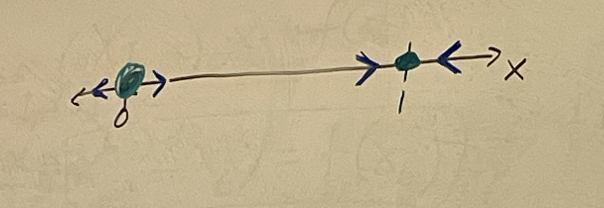
\includegraphics[width=0.5\linewidth]{Screen Shot 2023-11-13 at 11.52.17 AM.png}
    \caption{phase line of $\frac{\partial N}{\partial t}$}
    %\label{fig:enter-label}
\end{figure}

$\frac{\partial N}{\partial t} < 0$ (shrinking) when $N < 0$ \\
$\frac{\partial N}{\partial t} > 0$ (growing) when $N > 0, N < 1$ \\
$\frac{\partial n}{\partial t} < 0$ (shrinking) when $N > 1$ \\

Therefore, 0 is an unstable and 1 is a stable equilibrium. 


\end{document}